% !TEX root = ../main.tex

\chapter{関連研究・関連作品}
\label{chp:second}

\section{Interactive Kaleidoscope}
\label{sec:eqn}

この研究 \cite{Bongers2011InteractiveKA}では，博物館にインタラクティブアートを展示し，
観客がどのように作品と関わるかを調査・分析している．実験に用いられた作品は，広い壁面への映像投影と，
センサーを備えた木製のインタラクションオブジェクトによって構成され，
観客の体の動きやオブジェクトの操作に応じて，投影される万華鏡映像が変化する．
また，この研究には3つの研究課題が設定されている．
\begin{enumerate}
    \item インスタレーションが観客を十分に引き込むか
    \item インタラクションの方法が観客にとって明確であるか
    \item 参加者がどの程度作品に関与するか
\end{enumerate}
である．\\
調査の結果，観客の約4分の1が実際に作品へ参加しており，参加者の中には数分間にわたって体験を続けるものも
確認された．また，作品への関わり方を観察した結果，観客は作品に気づいた後すぐに参加するのではなく，
周囲を観察したり，他の参加者の行動を見たりしながら，段階的に作品への関与を深めていくことが示された．
さらに，参加者同士が協力して作品を操作するなど，作品を介した交流も確認された．\\
以上の分析結果を踏まえ，同研究では観客がインタラクティブ・インスタレーションに関わる過程を
以下の5段階に分類したインタラクションモデルを提案している．
\begin{enumerate}
    \item Ignore：作品に気づかない
    \item Notice：作品の存在に気づく
    \item Observe：作品を観察する
    \item Involvement：作品に参加する
    \item Engagement：作品に没入する
\end{enumerate}
この研究は，インタラクティブ参品における観客の関与を，作品への気づきから参加，
没入に至るまでの過程として捉えている点で，本研究におけるインタラクション設計および作品評価の参考となる．
特に本研究では，他者との関わりをきっかけとして身体映像が変化するため，参加者がどのように作品を認識し，
他者との関わりへと移行していくのかを考える上で参考になる．

\section{Boundary Functions}

Boundary Functions \cite{webpage6}は，床面に投影される映像を用いて，ギャラリー内にいる人々の
パーソナルスペースを可視化したインタラクティブアート作品である．図\ref{fig:gazou3}に実際の展示風景を示す．

\begin{figure}[H]
    \centering
	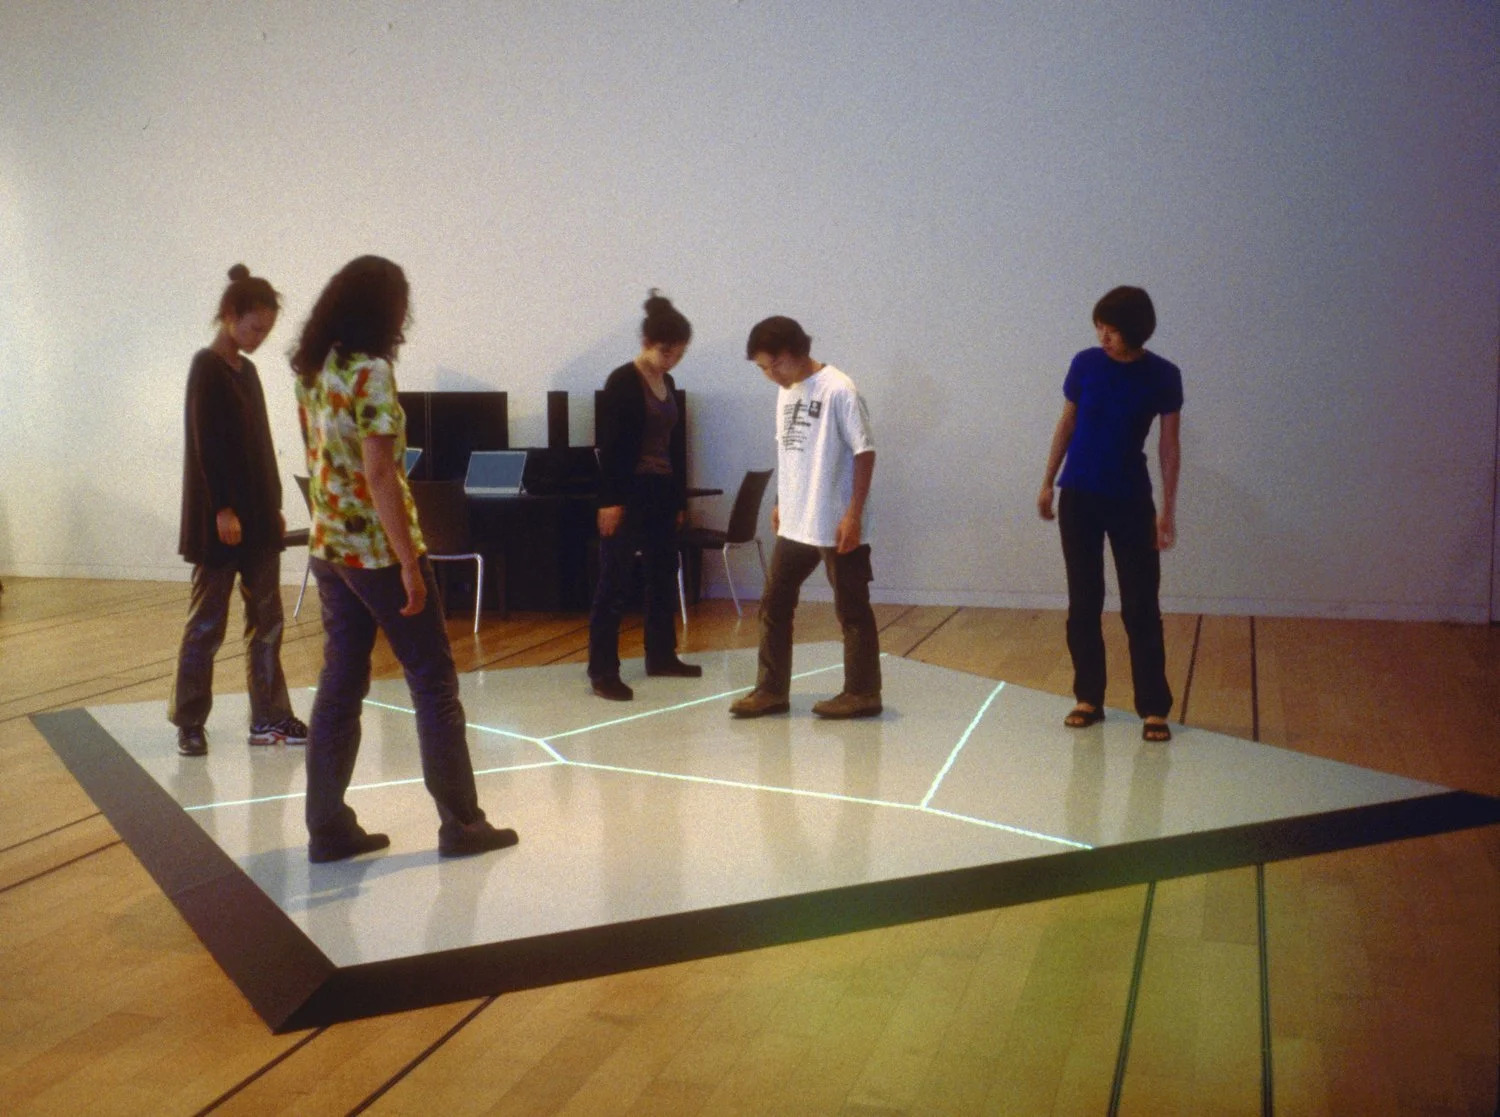
\includegraphics[width=6.4cm]{fig/gazou3.jpg}
    \caption{Boundary Functions}
    \label{fig:gazou3}
    {\small 出典：Scott Snibbe, ``Boundary Functions''．}
\end{figure}

空間内に1人しかいない場合，床面の映像には何も表示されない．2人になると，両者の間に1本の線が
投影され，床を二分し，2人の動きに合わせて線が動的に変化する．3人以上になると，床はセル上の
領域に分割され，各領域は，その内部にいる人に誰よりも近いという性質を持つ．\\
パーソナルスペースは，他者との関係性の中でしか存在せず，当人の意志だけでは制御しえない形で
変化していく．床面に線を投影することで，個人間に存在する目に見えない境界が，動的で具体的な形
として提示される点がこの作品の特徴である．また，この作品は他者が物理的にその場にいなければ
一切機能しない点も重要であり，1人では成立しえない体験として設計されている．\\
本研究とBoundary Functionsは，自己に関わる何らかの性質が，他者との関係性の中で
変化していくことを可視化する点，1人では作品が成立しない構造を持つという点で共通する．
しかし，Boundary Functionsが対人間の空間的距離を可視化するのに対し，本研究は自己の内的な
変化を可視化する点で異なる．

\section{本研究の位置付け}
\label{sec:bib}

以上の関連研究・関連作品との比較から，本研究の位置付けは，可視化する対象が空間的な距離
ではなく，接触を契機として生じる自己の内的な変化とする点にある．\\
こうした設計の背景には，二コラ・ブリオーの関係性の美学 \cite{book5}の考え方がある．
ブリオーは作品を独立したモノとしてではなく，人と人との関わりそのものを生み出す装置として捉え，
そこで生まれた関係性そのものを作品とする考えを示している．この考えに基づけば，
対人関係を扱う作品において重要なのは，関係が持つ性質を表現の構造そのものに反映させることだと
考えられる．\\
本研究は，この考え方に基づき，参加者間の身体的接触と，それによって生じる変化の持続性を
作品の中心的な構造として設計する点において，既存の関連研究・関連作品とは異なる新規性を持つ．

\chapter{研究内容}
\label{chp:third}

\section{システム要件}

1.2で述べた目的を達成するために，本研究では次の三つの要件を満たすシステムの構築を目指す．\\
第一に，参加者間の接近・接触を検出できることである．第二に，検出した接触の度合いや
持続時間に応じて，両者の身体イメージにそれぞれの変化が生じることである．
第三に，生じた変化が接触の終了とともに消えるのではなく，接触時間の長さに応じてその影響が
残り続け，痕跡として残ることである．\\
これらの要件を満たすシステムを通じて，参加者が相互作用を繰り返し経験する中で，
他者と関わる前後で自己の変化をどう感じたか，また自分自身が他者にどのような影響を与えたかを
振り返ることができるような体験を設計する．

\section{提案手法}
本研究では，ビジュアルプログラミング環境であるTouchDesignerを用いて提案手法を実装する．
Webカメラの映像から取得した参加者の身体の位置情報をもとに，
両者の身体イメージに局所的な歪みを生じさせる．歪みは接触した部位を中心として発生し，
接触時間が長いほど，その影響が強く，かつ強く残るように設計する．\\
生じた歪みは単一のフレームで消失するのではなく，フィードバックループの仕組みを用いて
映像上に蓄積させる．これにより，一度生じた変形が完全には元に戻らず，
次の接触による変形と重なる．この蓄積によって，自己変容が一度きりの出来事ではなく，
多くの関わり合いによって生じる過程であることを，視覚的に表現する．\\
なお，両者の身体イメージにおける変形の生じ方は対称である必要はなく，
それぞれの接触の仕方に応じて非対称に変化しうるものとして設計する．
これは，他者との関わりにおいて，影響を与える度合いと受ける度合いが必ずしも等しくない
という考えに基づく．

\chapter{プロトタイプの実装}
\label{chp:force}

\section{開発環境}
プロトタイプの開発には，ビジュアルプログラミング環境であるTouchDesignerを使用した．
全身をトラッキングする前に，実験的に手の情報だけを取得することにし，トラッキングには，
Googleが提供する機械学習フレームワークのMediaPipeを用いている．

\section{実装内容}
処理の流れは，MediaPipeによる手の動きの取得，歪みエフェクトの生成，
歪みエフェクトの持続という3段階から構成される．現時点では以下の機能を実装済みである．\\
\begin{enumerate}
    \item 人差し指の動きの追従（片手での検出から両手での検出へ拡張）
    \item 接触部位を中心とした歪みエフェクトの生成
    \item Feedback TOPを用いた歪みの持続ループの実装（一定時間，エフェクトの影響が映像上に残る仕組み）
\end{enumerate}

\section{現時点の動作}
現時点のプロトタイプでは，図\ref{fig:gazou1}のように両手の人差し指の位置をリアルタイムに取得し，
指先の動きに合わせて局所的な歪みを映像上に生成できることを確認している．
また，生じた歪みが一定時間映像上に残り続けることも確認済みである．\\
一方で，以下の点は未実装であり，今後の課題として残されている．
\begin{enumerate}
    \item 全身を検出対象とするシステムが構築できていない
    \item 複数人を同時に検出する処理に対応していない
    \item 意図した歪みの質感・強度を十分に再現できていない
\end{enumerate}

 \begin{figure}[H]
     \centering
	 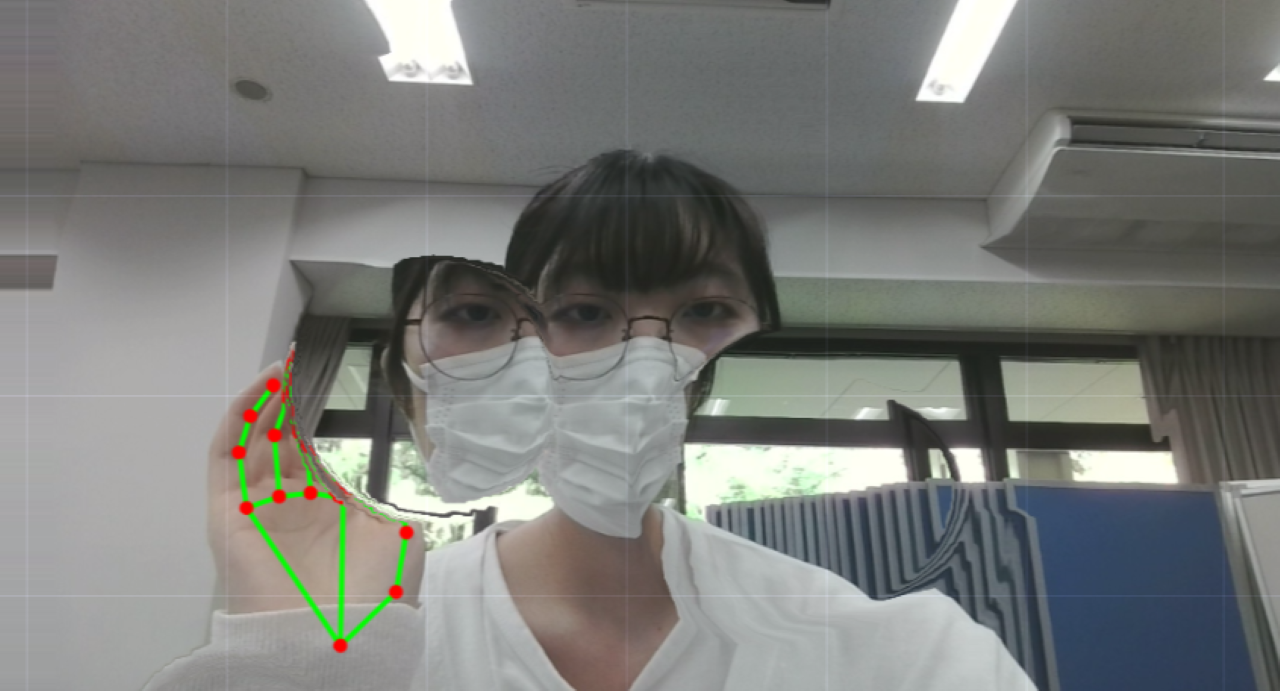
\includegraphics[width=6.4cm]{fig/gazou1.png}
     \caption{プロトタイプの現状}
     \label{fig:gazou1}
 \end{figure}

 \chapter{今後の課題}

 現時点のプロトタイプは，対象者1人の手指のみの検出という限られた範囲での実装にとどまっている．\\
そのため，今後は以下の課題に取り組む．\\
第一に，手指の身のトラッキングから全身の骨格情報を用いたトラッキングへと拡張し，
身体全体が変形する表現を実現する．第二に，複数人が同時に関わり合う場合に対応するシステムを実現する．
第三に，接触の度合いや持続時間に応じた歪みの強度・表現を調整し，図\ref{fig:gazou2}のように意図した表現を実現する．\\
これらの技術的な拡張と並行して，対人関係における自己変容や相互作用について扱う社会心理学について学び，
本作品が可視化しようとする自己変容の概念をより明確なものとして固めていく．

 \begin{figure}[H]
     \centering
	 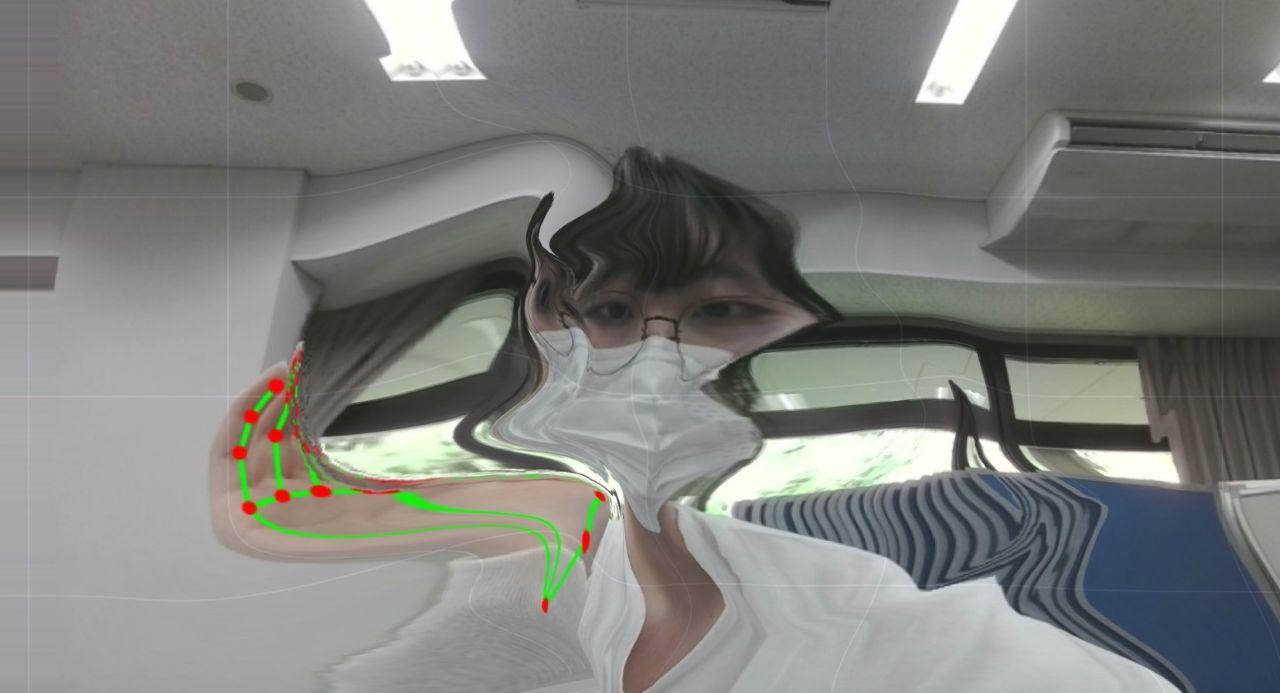
\includegraphics[width=6.4cm]{fig/gazou2.jpg}
     \caption{理想とする表現}
     \label{fig:gazou2}
 \end{figure}

